\documentclass[14pt]{extarticle}

\usepackage{geometry}
\usepackage{amsmath,amsthm,amssymb}
\usepackage[utf8]{inputenc}
\usepackage[T1,T2A]{fontenc}
\usepackage{bold-extra}
\usepackage[english,russian]{babel}
\usepackage{indentfirst}
\usepackage{graphicx}
\graphicspath{ {images/} }
\usepackage{float}
\usepackage{listings}
\usepackage{lmodern}
\usepackage{appendix}
\usepackage{braket}
\usepackage{cite}
\usepackage[nottoc,numbib]{tocbibind}

\geometry{
a4paper,
left = 20mm,
right = 15mm,
bottom = 20mm,
top = 20mm,
}
\renewcommand{\rmdefault}{ftm} % TimesNewRoman
\renewcommand{\baselinestretch}{1.5} 

\begin{document}

\begin{titlepage}
	\begin{center}
		\small{ФЕДЕРАЛЬНОЕ ГОСУДАРСТВЕННОЕ БЮДЖЕТНОЕ ОБРАЗОВАТЕЛЬНОЕ}\\ 
			УЧРЕЖДЕНИЕ ВЫСШЕГО ОБРАЗОВАНИЯ\\
			«МОСКОВСКИЙ ГОСУДАРСТВЕННЫЙ УНИВЕРСИТЕТ\\
			имени М.В.ЛОМОНОСОВА»\\
		\hfill \break
		ФАКУЛЬТЕТ ВЫЧИСЛИТЕЛЬНОЙ МАТЕМАТИКИ И КИБЕРНЕТИКИ\\
		КАФЕДРА СУПЕРКОМПЬЮТЕРОВ И КВАНТОВОЙ ИНФОРМАТИКИ\\
		\vfill
		ЗАДАНИЕ 2 \\
		\textbf{<<АНАЛИЗ БЛОЧНОГО АЛГОРИТМА МАТРИЧНОГО УМНОЖЕНИЯ С ПОМОЩЬЮ СИСТЕМЫ PAPI>>}\\
	\end{center}	
	\vfill
	\begin{flushright}
		Выполнил студент \\
		группы м118:\\
		Пухов Д. Н.\\
		{\hspace{3cm}}
	\end{flushright}
	
	
	\begin{center}
		Москва \\
		2017 
	\end{center}
	
	\thispagestyle{empty}

\end{titlepage}





\section*{Формулировка задачи} 
Реализовать последовательный алгоритм блочного матричного умножения и оценить влияние кэша на время выполнения программы. Дополнить отчёт результатами сбора информации с аппаратных счётчиков, используя систему PAPI.

\section*{Описание алгоритма}
Уравнение $ C = A \cdot B $, где $ A = n \times m $, $ B = m \times h $, $ C = n \times h $, можно переписать следующим образом:
\begin{equation*}
c_{ij} = \sum \limits_{k=0}^{k=m-1} a_{ik} b_{kj}, \quad i = \overline{0,n-1}, \quad j = \overline{0,h-1},
\end{equation*}
что соответствует следующему коду на языке C:
\begin{lstlisting}[language=C]
for(int i=0; i<n; ++i)
	for(int j=0; j<h; ++j)
		for(int k=0; k<m; ++k)
			C[i][j] += A[i][k] * B[k][j];
\end{lstlisting}

Это прямой алгоритм умножения матриц. Идея блочного алгоритма заключается в повышении эффективности работы кэша, а именно в улучшении пространственной локальности данных: в кэш загружаются небольшие блоки умножаемых матриц, с ними проводятся вычисления, следующие блоки загружаюся в кэш и т.д.
В данной работе оптимизируется только кэш первого уровня - L1.

Программа производит расчёты на числах одинарной точности для блока размером $32 \times 32$ в режимах ijk, ikj и для блока оптимального размера в режиме ijk.

\subsection*{Определение оптимального размера блока}
Ядро процессора Intel Core i5 3230M имеет L1d кэш размером 32 KiB.
Размер линии кэша равен 64 B.
Размер числа одинарной точности равен 4 B.
В кэше нужно хранить 3 блока оптимального размера $b$ (измеряем в количестве чисел, а не в байтах).

Таким образом, $ 3b^2 <= \frac{32*1024}{4} $, откуда $b = 52$.

\subsection*{Используемый код}
\begin{lstlisting}[language=C]
void square_dgemm_ijk_with_call_ijk(float* A, float* B, float* C,
                                        int n, int bsz)
{
    for(int i=0; i<n; i+=bsz)
    {
        const int i_offset = i*n;
        const int M = min(bsz, n-i);
        for(int j=0; j<n; j+=bsz)
        {
            const int N = min(bsz, n-j);
            for(int k=0; k<n; k+=bsz)
            {
                const int K = min(bsz, n-k);
                calculate_block_ijk(A+i_offset+k, B+k*n+j,
                		C+i_offset+j, M, N, K, n);
            }
        }
    }
}

static void calculate_block_ijk(float* A, float* B, float* C,
                                    int M, int N, int K, int n)
{
    for(int i=0; i<M; ++i)
    {
        const int i_offset = i*n;
        for(int j=0; j<N; ++j)
        {
            float cij = 0.0;
            for(int k=0; k<K; ++k)
                cij += A[i_offset+k] * B[k*n+j];
            C[i_offset+j] += cij;
        }
    }
}
\end{lstlisting}

\section*{Описание программы}
\subsection*{Запуск}
Программа использует Makefile и не предусматривает различных сценариев запуска.
Для обработки данных требуется запустить скрипт report.py.

\subsection*{Формат записи в файл}
Запись осуществляется в два файла из соображений удобства записи (а не чтения) в формате csv. Однако файлы имеют расширение txt ("../res/results1.txt" и "../res/results2.txt"). При обработка они сливаются другой сторонней программой в единый csv файл.

Формат записи: indices,n,bsz,events,time,\\
где indices = ijk или ikj --- порядок индексов внутри блока,\\
n --- размер матрицы,\\
bsz --- размер блока,\\
events --- одно или несколько значений счётчиков (зависит от аргумента функции тестирования),
time --- время в секундах.

Пример первых двух строк:
\begin{lstlisting}
indices,size,bsz,PAPI_L1_DCM,PAPI_L2_DCM,PAPI_TOT_CYC,time
ijk,1000,32,10101668,6251000,9925367478,3.113803
\end{lstlisting}
Здесь events содержит три счётчика.

Все расчёты проводились без усреднения.



\section*{Результаты}
Ожидаемое число промахов должно быть одинаковым для ijk, ikj $32 \times 32$, поскольку блок матрицы так или иначе полностью загружается в кэш. Число промахов для оптимального размера блока (52 для данного процессора) должно быть больше, чем для блока $32 \times 32$!

Я рассуждаю по следующей модели. Поскольку данные загружаются в L1 линиями длиной 64 байта, или 16 чисел одинарной точности, то блок $32 \times 32$ требует $32 \times 2$ обращений в память, причём линии кэша используются максимально эффективно. Когда блок имеет размер $52 \times 52$, требуется $52 \times 4$ обращений в память, причём каждое третье обращение загружает линию кэша лишь частично (52-16-16-16=4 числа должны быть загружены, вместе с ними загружается "мусор" длиной 16-4=12 чисел).

Итоговая формула числа промахов кэша определяется числом матриц, количеством блоков внутри одной матрицы и количеством промахов кэша при загрузке одного блока:
\begin{equation*}
L1\_DCM \le 3 \times \left( \big \lceil \frac{matrix size}{block size} \big \rceil \right)^2 \times b \times \lceil \frac{block size}{cache line size} \rceil .
\end{equation*}

Формула учитывает только холодные промахи кэша, т.е. подразумевается, что все данные помещаются в кэш и не замещаются данными других программ (ОС, например, может что-то хранить в кэше). Первое условие должно выполняться, поскольку мы соответствующим образом вычислили размер блока. Второе условие может быть невыполненным, это нужно дополнительно изучить.

Возможные причины несоответствия графиков формуле: неверные измерения, архитектурные особенности работы кэша, особенности работы счётчиков, неверная обработка данных.

Также глубоко неясно, почему общее число операций с плавающей запятой зависит от порядка индексов и размера блока (операций всё равно $n^3$).

\begin{figure}[H]
	\centering
	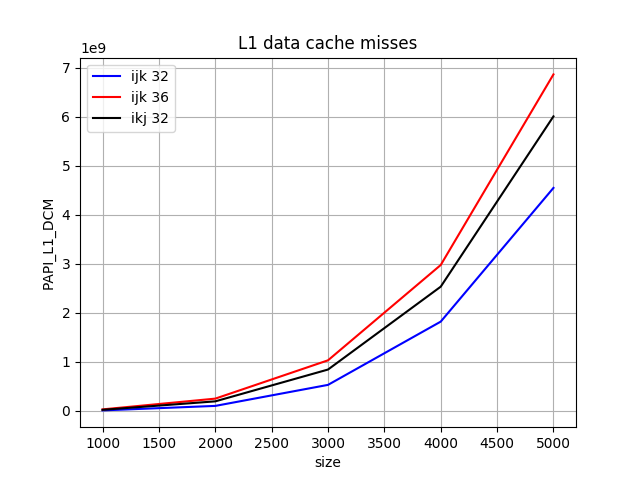
\includegraphics[scale=1]{Figure_1}
\end{figure}

\begin{figure}[H]
	\centering
	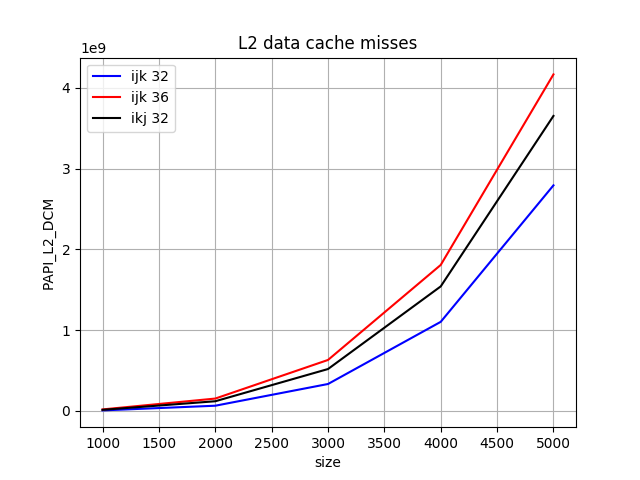
\includegraphics[scale=1]{Figure_2}
\end{figure}

\begin{figure}[H]
	\centering
	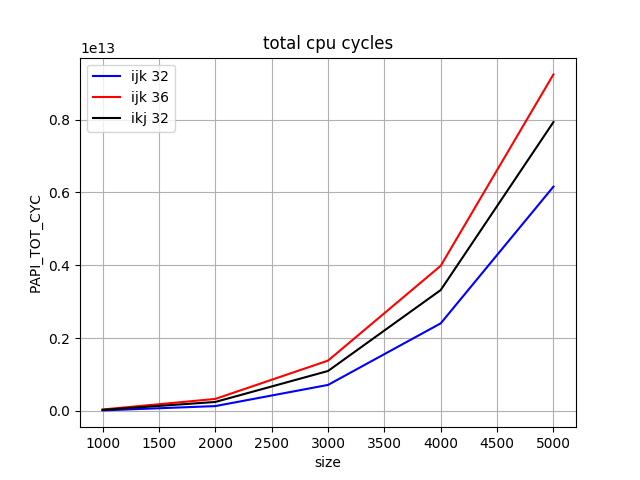
\includegraphics[scale=1]{Figure_3}
\end{figure}

\begin{figure}[H]
	\centering
	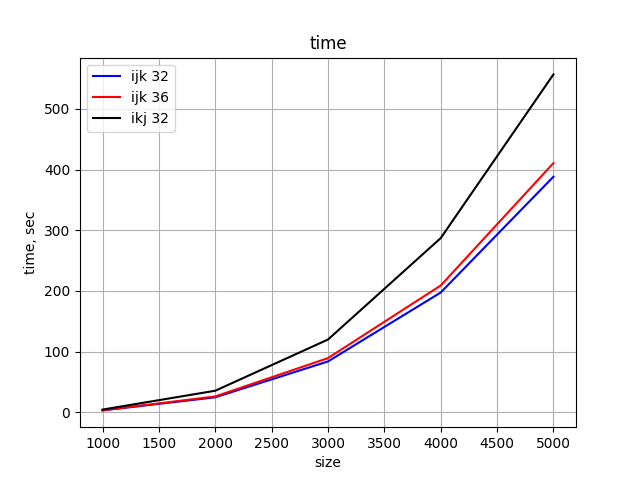
\includegraphics[scale=1]{Figure_4}
\end{figure}

\begin{figure}[H]
	\centering
	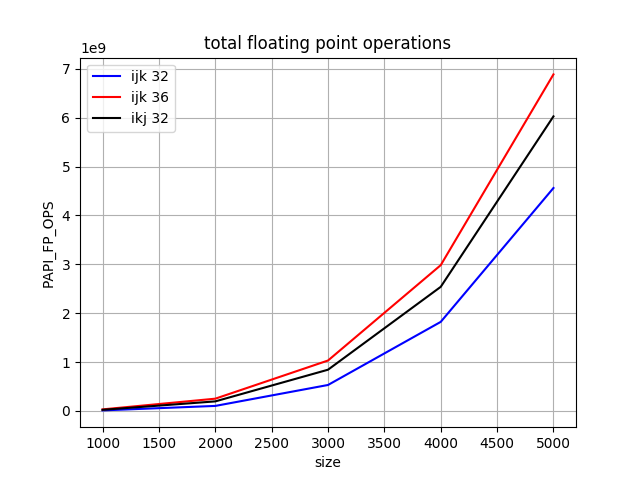
\includegraphics[scale=1]{Figure_5}
\end{figure}

\begin{figure}[H]
	\centering
	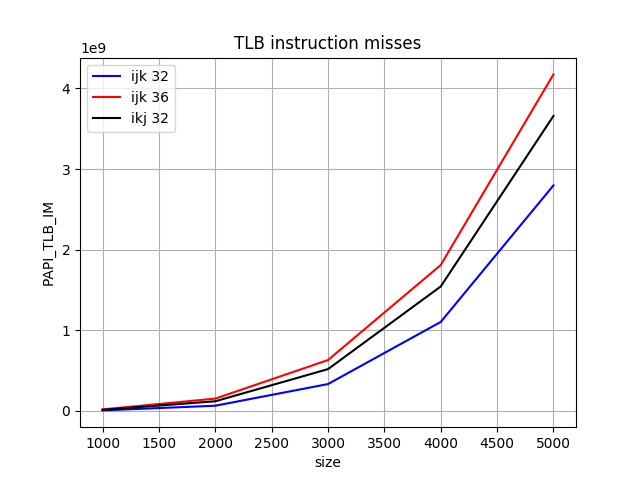
\includegraphics[scale=1]{Figure_6}
\end{figure}

\begin{figure}[H]
	\centering
	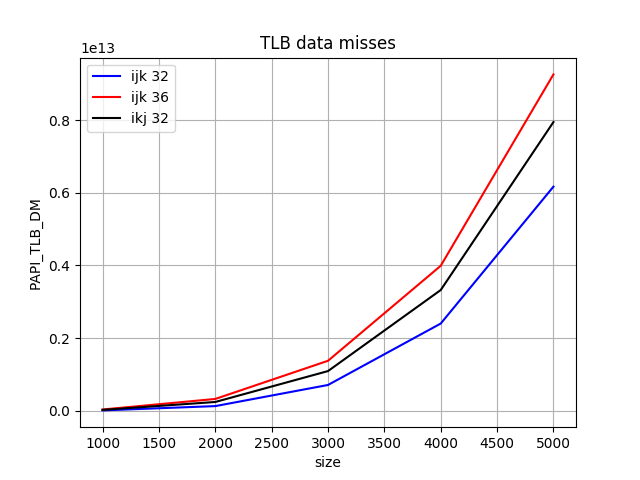
\includegraphics[scale=1]{Figure_7}
\end{figure}

\end{document}\grid
